%% Impact de la hiérarchie mémoire sur les performances parallèles - Loic Poncet
%% Rapport rédigé à l'aide de Texmaker

\documentclass[a4paper,12pt]{report}
\usepackage[utf8]{inputenc}
\usepackage[french]{babel} 
\usepackage[left=2cm,right=2cm,top=2cm,bottom=2cm]{geometry} % ajuste la taille des marges
\usepackage{url} 	  % permet d'ajouter des url
\usepackage{setspace}
\usepackage{tgtermes}
\usepackage{fancyhdr} % permet de changer les en-tête
\usepackage{graphicx} % permet l'insertion d'images
\usepackage{titlesec}
\usepackage{hyperref} % table des matières clicable
\usepackage{amsmath}  % pour matrices
\usepackage{textcomp}
\usepackage{enumitem} % permet de changer le format des listes
\usepackage{chngcntr} % permet une continuité des notes de bas de page à travers les chapitres
\usepackage{listings}

%%configuration de listings
\lstset{
language=c,
basicstyle=\ttfamily\small, %
identifierstyle=\color{black}, %
keywordstyle=\color{black}, %
stringstyle=\color{black}, %
commentstyle=\it\color{green!95!yellow!1}, %
columns=flexible, %
tabsize=2, %
extendedchars=true, %
showspaces=false, %
showstringspaces=false, %
numbers=left, %
numberstyle=\tiny, %
breaklines=true, %
breakautoindent=true, %
captionpos=b
}

\usepackage{xcolor}

\definecolor{Zgris}{rgb}{0.87,0.85,0.85}

\newsavebox{\BBbox}
\newenvironment{DDbox}[1]{
\begin{lrbox}{\BBbox}\begin{minipage}{\linewidth}}
{\end{minipage}\end{lrbox}\noindent\colorbox{Zgris}{\usebox{\BBbox}} \\
[.5cm]}

\counterwithout{footnote}{chapter}
 

\AddThinSpaceBeforeFootnotes % Permet de mieux respecter les règles de typographie française 
\FrenchFootnotes % Permet de mieux respecter les règles de typographie française 

\hypersetup{ % gestion des hyperliens
    colorlinks,
    citecolor=blue,
    filecolor=black,
    linkcolor=black,
    urlcolor=black
}


\titleformat{\chapter}[hang]{\bf\LARGE}{\thechapter}{2pc}{} % change le format des titres de chapitres

\titleformat{\section}[hang]{\bf\Large}{\thesection}{2pc}{} %change le format des titres de sections

\titlespacing*{\chapter}{0pt}{0pt}{40pt}

\pagestyle{fancy} % modifie le style des pages
\renewcommand\headrulewidth{1pt}
\fancyhead[L]{}
\fancyhead[R]{\textit{Impact de la hiérarchie mémoire sur les performances parallèles}}

\fancypagestyle{plain}{}


\begin{document}

\begin{titlepage}

\begin{center}
	\begin{flushright} % logo UGA
		
\includegraphics[scale=0.8]{logo-uga.png}\\[1.5cm]
	\end{flushright}
	\large{Université Grenoble Alpes\\
		   Département Licence Sciences \& Technologie\\[1.5cm]}
	
	\textbf{\LARGE{RAPPORT DE STAGE\\}}
	
	% titre du rapport
	\rule{\linewidth}{0.5mm} \\[0.4cm]
	\textbf{\LARGE{Impact de la hiérarchie mémoire sur les performances parallèles}}\\[0.4cm]
	\rule{\linewidth}{0.5mm} \\[0.4cm]
	
	\textbf{\textit{	PONCET Loic\\[0.8cm]}}
	
\includegraphics[scale=0.15]{LIG_coul.jpg}\\[0.8cm] % logo LIG
\end{center}

\begin{flushleft}
	Laboratoire d'accueil : Laboratoire d'Informatique de Grenoble\\
	Directeur du laboratoire : Eric Gaussier\\
	Responsable du stage : Guillaume Huard\\[1.0cm]
\end{flushleft}

\begin{flushright}
	Licence Sciences et Technologie 2\up{ème} année - Mathématiques et 		Informatique\\
	Année Universitaire : 2015/2016
\end{flushright}

\end{titlepage}

\pagenumbering{roman}

\begin{onehalfspace}

\chapter*{Remerciements}

Tout d'abord, j'adresse mes remerciements à l'Université Grenoble Alpes ainsi qu'au Laboratoire d'Informatique de Grenoble qui m'ont permis d'effectuer ce stage.\\

Je remercie Guillaume Huard, mon maître de stage, pour m'avoir donné ma chance et pour avoir toujours répondu présent lorsque j'avais besoin de ses conseils. Sa gentillesse, la confiance qu'il m'a accordée ainsi que le savoir qu'il m'a transmis pendant ces 6 semaines ont grandement contribué à la réussite sur le plan personnel de ce stage.\\

Mes remerciements vont également à Orianne Soto ainsi qu'à Annie Simon pour avoir géré les parties administratives de mon stage.\\

Enfin, j'exprime toute ma gratitude envers toutes les personnes avec qui j'ai pu collaboré au sein du LIG, en particulier à:
\begin{itemize}[label=\textbullet]
\item Michael Picard, autre stagiaire d'excellence, pour l'aide qu'il m'a apportée ainsi que pour avoir partagé avec moi ce qu'il avait appris au cours de son stage,
\item l'ensemble des chercheurs des équipes POLARIS et DATAMOVE,
\item Lucas, Mathieu, Piat et Thomas avec qui j'ai partagé le bureau 424, qui m'ont accueilli chaleureusement et qui n'ont pas hésité à donner de leur temps pour m'aider et me faire découvrir des outils que je ne maîtrisais pas.
\end{itemize} 

\renewcommand\contentsname{\bf\hfill Table des matières \hfill}
\tableofcontents

\pagestyle{fancy}

	

\chapter{Introduction}

\pagenumbering{arabic}

\section{Environnement}

J'ai été accueilli durant ces six semaines de stage au Laboratoire d'Informatique de Grenoble (LIG). Le LIG est l'un des principaux laboratoires de recherche en informatique de Grenoble, il contribue au développement des sciences informatiques et tente de relever les défis technologiques d'aujourd'hui et de demain.\\

Mon stage s'est déroulé au sein de l'équipe POLARIS, l'une des 24 équipes de recherche du LIG\footnote{\url{https://www.liglab.fr/presentation/equipes}},  dont le projet est d'étudier les performances des très grands systèmes distribués à travers des simulations, des modélisations ou encore des optimisations d'algorithmes adaptés. De ce fait, j'ai pu bénéficier des connaissances des membres de l'équipe dans le domaine du calcul parallèle, mais également sur les impacts de la hiérarchie mémoire sur les performances.\\

L'ensemble des résultats présentés dans ce document ont été obtenu avec la configuration suivante (en résumé):

\begin{center}
\begin{tabular}{|c|}
\hline
	HP\textsuperscript\textregistered Z800 Workstation \\
	Processeur Intel\textsuperscript\textregistered Xeon\textsuperscript\textregistered  		E5620 2.40GHz \cite{proc}\\
	Hyper-threading désactivé\\
	Compilateur GCC version 5.3.1 \\
\hline
\end{tabular}
\end{center}

Pour plus d'informations sur ma configuration ainsi que sur les paquets installés sur ma machine voir le dépôt Github du stage: \url{https://github.com/LoicPoncet/Stage-LIG-Poncet}

\section{Présentation du sujet et motivations}

L'intitulé exact de mon sujet de recherche est: \textbf{\textit{"Impact de la hiérarchie mémoire sur les performances parallèles"}}. Un sujet portant à la foi sur l'architecture des ordinateurs mais également sur le parallélisme en informatique. 

\subsection{Qu'est-ce que le parallélisme?}
On désigne par parallélisme le fait de réaliser plusieurs calculs simultanément sur un ordinateur, cela nécessite une machine possédant plusieurs coeurs, ou bien plusieurs processeurs. Ainsi, lorsqu'un programme s'exécute en parallèle, différentes portions du code, ou bien différents calculs pourront être exécutés au même moment.\\ 

Le parallélisme s'est développé pour répondre à deux besoin bien spécifiques: améliorer la puissance de calcul des ordinateurs et réduire leurs coût \cite{ref2}.

Il s'agit d'une notion au combien importante aujourd'hui dans le domaine de l'informatique. Les calculs réalisés en parallèle permettent un gain de performances considérable par rapport aux calculs effectués de manière classique, si bien qu'ils sont aujourd'hui utilisés dans bon nombre de domaines.

\section{Structure du rapport}

Ce rapport sera divisé en deux grandes parties. La première explicitera l'importance de la gestion de la mémoire dans un programme et son impact sur les performances. Cette partie sera plus "technique" et permettra d'introduire certaines notions importantes pour la suite. La deuxième partie sera la partie centrale de ce rapport. Elle traitera du calcul parallèle, mon apprentissage de celui-ci et reprendra les grandes idées de la première partie en les appliquant aux architectures parallèles.     
\chapter{L'importance d'une bonne gestion de la mémoire}

J'ai consacré une partie importante de mon stage à me renseigner sur l'architecture des ordinateurs et principalement comment était organisée la mémoire à l'intérieur de ces derniers. Bien comprendre comment l'ordinateur gère la mémoire est primordial pour obtenir de bonnes performances lors de l'exécution de nos programmes \cite{Drepper} (surtout lorsque plusieurs threads s'exécutent en même temps). Dans ce rapport, nous allons nous intéresser en particulier à la mémoire cache.

\section{La mémoire cache}

La mémoire cache fut développée dans les ordinateurs afin de diminuer les temps d'accès aux données stockées dans la mémoire principale. Ainsi, lorsque le processeur a besoin de données stockées dans la mémoire principale, il va réaliser une copie de celles-ci afin de les rendre plus rapidement accessibles s'ils venaient à en avoir besoin peu après. Cette amélioration est rendue possible par deux grands principes: les principes de localité spatiale et temporelle. En effet lorsqu'un programme utilise des données ou exécute des instructions, il tend à utiliser très prochainement des données ou instructions proches dans la mémoire de celles actuellement utilisées (un cas typique est la boucle \textbf{For} où les mêmes instructions seront exécutées encore et encore). \\

Le cache est généralement composé de 2 ou 3 niveaux que l'on note L1, L2 et L3. Le niveau L1, qui est le plus petit mais le plus rapidement accessible, est la plupart du temps séparé en deux parties dans un souci d'optimisation: L1d pour les copies de données et L1i pour les copies d'instructions. Le temps que met le processeur à accéder aux données présentes dans un niveau de cache croit plus ce dernier est élevé. En contrepartie, la capacité de stockage des différents niveaux de cache croit également de la même façon. \\

Afin de tenir compte du principe de localité évoqué précédemment, ce n'est pas un mot mémoire qui est chargé dans le cache mais une "ligne de cache" contenant plusieurs mots. Aujourd'hui standardisée, la taille d'une ligne de cache est de 64 octets. 

\section{Comment optimiser l'utilisation du cache}\label{Section:2.2}

En tenant compte  de ce qui a été évoqué précédemment, on peut identifier quelles sont les bonnes attitudes à adopter pour que nos programmes soient plus efficaces. Prenons l'exemple du petit programme suivant. 


\begin{DDbox}{\linewidth}
\begin{lstlisting}
#include <stdio.h>
#include <stdlib.h>

int main(){
	int tab[1000][1000];
	int i,j;

	for(i=0;i<1000;i++){
		for(j=0;j<1000;j++){
			tab[i][j] = 0;
		}
	}

	return(0);
}
\end{lstlisting}
\end{DDbox}

Dans celui-ci le tableau d'entiers à deux dimensions est parcouru séquentiellement, comme nous pouvons le voir dans la \hyperref[figure:2.1]{Figure 2.1} sur le tableau de gauche. Dans cette configuration, le processeur profite des données en cache. En effet, lorsqu'il commence à parcourir une nouvelle ligne, il extrait une ligne de cache de la mémoire principale. En considérant qu'un entier est codé sur 32 bits soit 4 octets, une ligne de cache contient donc 16 cases de notre tableau. Le processeur va donc charger des données présentes dans la mémoire cache pendant 16 itérations. \\
Supposons maintenant que nous inversons l'ordre des boucles, le schéma de parcours est à présent celui du tableau de droite de la \hyperref[figure:2.1]{Figure 2.1}. Dans cette configuration, nous ne profitons plus du cache puisque que les données chargées successivement par le processeur sont très éloignées dans la mémoire ce qui l'oblige à extraire à chaque fois une ligne de cache de la mémoire principale pour au final très peu l'utiliser. Cette version du programme est en moyenne environ 3 fois plus longue à exécuter que la précédente. 

\begin{figure}[ht]

	\begin{center}
	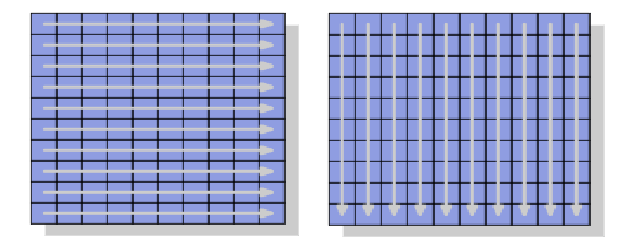
\includegraphics[scale=0.7]{tableaux.png} 
	\end{center}
	\caption{Différentes façons de parcourir un tableau}
	\label{figure:2.1}

\end{figure}


\chapter{Les calculs parallèles}

Mon apprentissage du calcul parallèle s'est fait en parallélisant un programme séquentiel calculant le produit de deux matrices à l'aide d'OpenMP \cite{ref1}. Avant d'expliquer comment fonctionne OpenMP et son utilisation, un bref rappel sur le calcul matriciel s'impose afin de comprendre en quoi il constitue l'exemple parfait pour aborder les calculs parallèles. 

\section{Pourquoi choisir le calcul matriciel}
Notons A et B deux matrices carrées de taille n dont nous souhaitons faire le produit. Notons C la matrice résultat, elle est également carrée de taille n. 
\begin{equation*}
\begin{pmatrix}
	a_{1,1} & \cdots & & \cdots & a_{1,n} \\
	\vdots & & \vdots & &\vdots \\
	a_{i,1} & \cdots & a_{i,k} & \cdots & a_{i,n} \\
	\vdots & & \vdots & & \vdots \\
	a_{n,1} & \cdots & & \cdots & a_{n,n} 
\end{pmatrix} 
\begin{pmatrix}
	b_{1,1} & \cdots & b_{1,j} & \cdots & b_{1,n} \\
	\vdots & & \vdots & &\vdots \\
	  & \cdots & b_{k,j} & \cdots &   \\
	\vdots & & \vdots & & \vdots \\
	b_{n,1} & \cdots & b_{n,j} & \cdots & b_{n,n} 
\end{pmatrix}
=
\begin{pmatrix}
	c_{1,1} & \cdots & & \cdots & c_{1,n} \\
	\vdots & & \vdots & &\vdots \\
	c_{i,1} & \cdots & c_{i,j} & \cdots & c_{i,n} \\
	\vdots & & \vdots & & \vdots \\
	c_{n,1} & \cdots & & \cdots & c_{n,n} 
\end{pmatrix}
\end{equation*}

Le calcul de l'élément (i,j) de la matrice C est réalisé à l'aide de la \hyperref[formule:3.1]{Formule 3.1}.
\begin{equation}
\large{C_{i,j} = \sum_{k=1}^{n} A_{i,k}*B_{k,j}} \label{formule:3.1}
\end{equation}

Nous voyons ici que l'élément (i,j) calculé est indépendant au niveau des calculs, de tous les autres éléments de la matrice résultat. Ainsi, l'entité réalisant le produit, que ce soit l'ordinateur ou un être humain, pourra calculer les éléments dans l'ordre qu'il souhaite sans que cela ait un effet sur la validité du résultat. C'est cela qui rend le produit matriciel intéressant pour appréhender le parallélisme. En effet, l'ordinateur, s'il dispose des ressources nécessaires, pourra calculer simultanément plusieurs éléments de la matrice résultat en assignant les calculs à plusieurs de ses processeurs plutôt que d'en laisser un seul effectuer l'ensemble des calculs.

\section{OpenMP}

OpenMP est une interface de programmation applicative permettant de paralléliser des programmes écrits en langage Fortran ou bien en C/C++. Il s'utilise à l'aide de directives destinées au compilateur que le programmeur ajoute à son programme séquentiel afin de distribuer le travail entre les différents processeurs ou coeurs en spécifiant quelles données doivent être partagées ou privées. Ceci rend son utilisation et son apprentissage extrêmement simple. Un exemple d'utilisation est donné dans la \hyperref[figure:3.1]{Figure 3.1} .    
\begin{figure}[hb]

	\begin{center}
	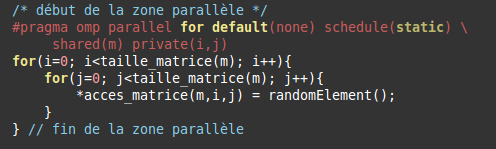
\includegraphics[scale=0.7]{exemple_OpenMP.png} 
	\end{center}
	\caption{Exemple d'utilisation d'un directive OpenMP}
	\label{figure:3.1}

\end{figure}
Dans cette figure nous pouvons voir comment est parallélisée une zone d'un programme à l'aide d'OpenMP. La directive "\#pragma omp parallel" permet d'indiquer au compilateur qu'il faut qu'une zone parallèle soit créée. L'ajout du "for" permet d'indiquer que la zone à paralléliser sera une boucle \textbf{For}. S'ajoutent ensuite différentes clauses qui permettent entre autre de choisir de quelle manière sera distribué le travail entre les différents threads ou encore combien de threads devront être utilisés. Enfin, le programmeur peut indiquer au compilateur quelles données seront partagées par les threads et celles dont chaque thread devra posséder une copie qu'il manipulera ensuite (le programmeur peut laisser le compilateur faire ce choix à sa place mais cela est vivement déconseillé). Une directive complète sera analysée plus en détail plus loin dans le rapport. \\
 
Le plus compliqué reste en fait d'identifier les zones d'un programme propices à une exécution parallèle. Ainsi, le programmeur devra de temps en temps changer un de ses algorithmes afin d'optimiser son programme pour le parallélisme.  


\section{Premiers algorithmes et résultats}

J'ai choisi de manipuler uniquement des matrices représentées en mémoire par des tableaux monodimensionnels. Dans ce type de structure les lignes de la matrice sont stockées les unes après les autres en mémoire. Ceci améliore grandement la localité de nos données tout en évitant de nombreuses indirections. \\

J'ai commencé par implémenter l'algorithme naïf permettant d'effectuer le produit de deux matrices (carrées dans mon cas). Celui-ci est donné en \hyperref[figure:3.2]{Figure 3.2} . Paralléliser ce programme fut relativement simple (c'est d'ailleurs la version parallèle qui est présentée).

Pour plus d'informations, se référer à la documentation d'OpenMP\footnote{\url{http://openmp.org/wp/openmp-specifications/}}

\begin{figure}[ht]

	\begin{center}
	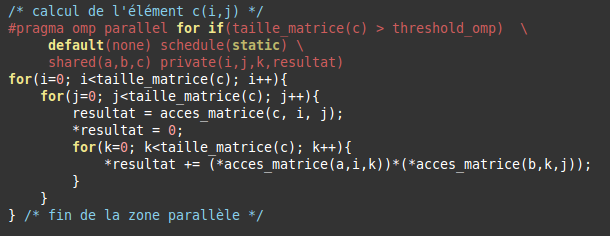
\includegraphics[scale=0.6]{algo_naif.png} 
	\end{center}
	\caption{Implémentation en C de l'algorithme naïf du produit matriciel}
	\label{figure:3.2}

\end{figure}

La \hyperref[figure:3.3]{Figure 3.3} présente une analyse des premiers résultats obtenus. Une série comparative des temps d'exécutions sur de très petites matrices lorsque les calculs sont réalisés en parallèle avec 8 threads et lorsqu'ils sont réalisés séquentiellement par 1 seul thread. 

\begin{figure}

	\begin{center}
	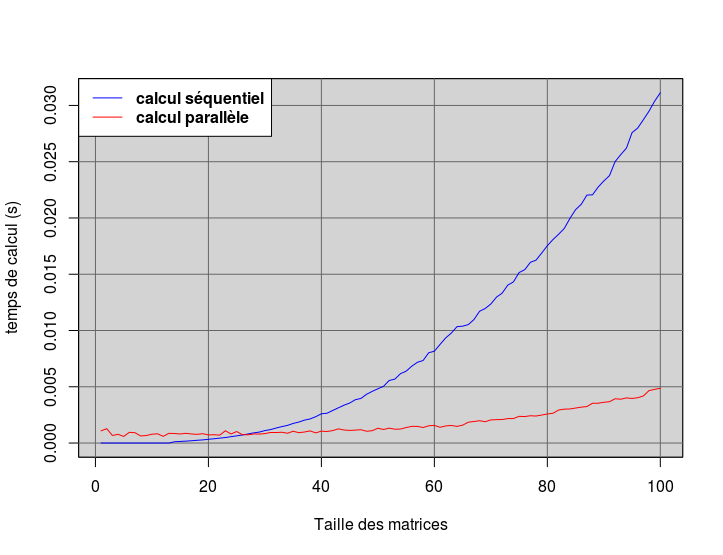
\includegraphics[scale=0.6]{premiers_resultats.png} 
	\end{center}
	\caption{Comparaison des temps de calculs sur des matrices de tailles 1x1 à 128x128}
	\label{figure:3.3}

\end{figure}

S'en est suivi une série de mesures permettant de mesurer l'accélération obtenue en utilisant les calculs parallèles en fonction du nombre de threads. 

Comme nous pouvons le voir dans cet algorithme, la matrice A est parcourue séquentiellement à l'inverse de la matrice B ce qui, comme nous l'avons vu dans la \hyperref[Section:2.2]{Section 2.2}, n'est pas une bonne chose. Pour chaque donnée de la matrice B requise par l'un des processeurs, et en considérant que nos matrices soient suffisamment grandes, une ligne de cache devra être extraite de la mémoire principale. De plus, cette dernière sera probablement évincée du cache avant d'être réutilisée. S'en suivent des performances médiocres. \\

L'une des façons d'améliorer les performances dans ce cas est de transposer la matrice B avant de réaliser les calculs afin de pouvoir la parcourir séquentiellement et donc d'utiliser les données présentes dans la mémoire cache. La \hyperref[formule:3.2]{Formule 3.2} donne le calcul de l'élément C(i,j) dans le cas où la transposée de la matrice B est utilisée.
\begin{equation}
\large{C_{i,j} = \sum_{k=1}^{n} A_{i,k}*{}^t \! B_{j,k}} \label{formule:3.2}
\end{equation}
 La \hyperref[figure:3.3]{Figure 3.4} présente une comparaison des temps de calculs avec les deux algorithmes en utilisant 8 threads. 

\begin{figure}[hb]

	\begin{center}
	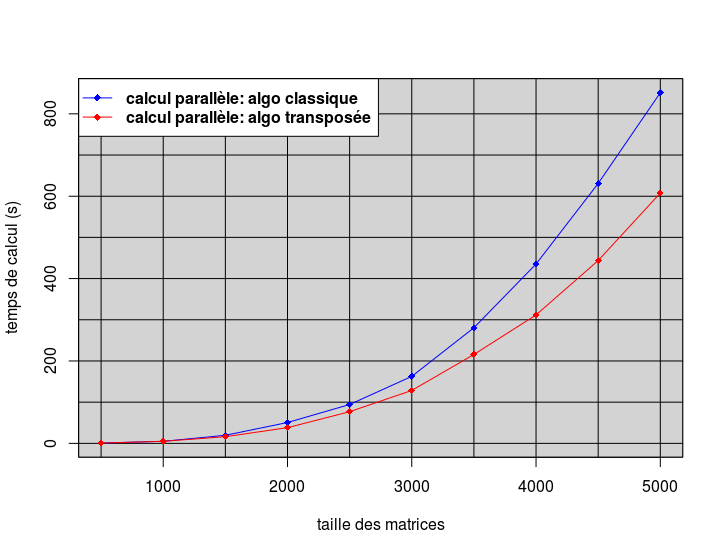
\includegraphics[scale=0.7]{para_transposee_500_5000.png} 
	\end{center}
	\caption{Comparaison des temps de calculs en fonction des algorithmes et de la taille des matrices}
	\label{figure:3.4}

\end{figure}

Nous pouvons voir que le surcoût d'opérations lié à la transposition de la matrice B est rapidement compensé par une bien meilleure utilisation du cache lors des calculs. Néanmoins, ces résultats restent peu satisfaisants car ils laissent présager des temps de calcul très longs pour de grosses matrices\footnote{des matrices dont la taille est inférieure à 10 000 sont considérées comme de petites matrices par les scientifiques étudiant les calculs parallèles}, la courbe des temps d'exécutions étant cubique! \\
C'est ici qu'une bonne utilisation de la mémoire peut nous faire gagner de nombreuses secondes. L'idée va être de séparer nos matrices en plusieurs blocs de tailles égales 




\end{onehalfspace}

\bibliographystyle{unsrt}
\bibliography{biblio}
\addcontentsline{toc}{chapter}{Bibliographie}


\end{document}